\chapter{Implementation}

%The implementation should look at any issues you encountered as you tried to implement your design. During the work, you might have found that elements of your design were unnecessary or overly complex, perhaps third party libraries were available that simplified some of the functions that you intended to implement. If things were easier in some areas, then how did you adapt your project to take account of your findings?

%It is more likely that things were more complex than you first thought. In particular, were there any problems or difficulties that you found during implementation that you had to address? Did such problems simply delay you or were they more significant? Your implementation might well be described in the same chapter as Problems (see below).

It is a good idea to first build a basic prototype.  Building a prototype will quickly highlight the main flaws in the initial design.  This is not the same as the intended final version and in this case is not even the same materials as I have chosen.  It does however conform the basic design but is made from much cheaper sourced components.  I already had an Arduino Uno (the basic prototyping model) from my interest int he technology before I attended university, so this was an easy component to get ym hands on quickly and is perfect for a prototype.  I had no chassis built or any materials to make one so I found a cheap and easy to assemble one online at a hobbyist electronics retailer.  This kit also included some very small DC motors with gearboxes and wheels, very convenient little package.  The Arduino alonge with the chassis kit and a small infrared sensors, a 9 volt battery and some jumper wires and a ptorotype was put together in an afternoon.
\begin{figure}[h]
\centering
        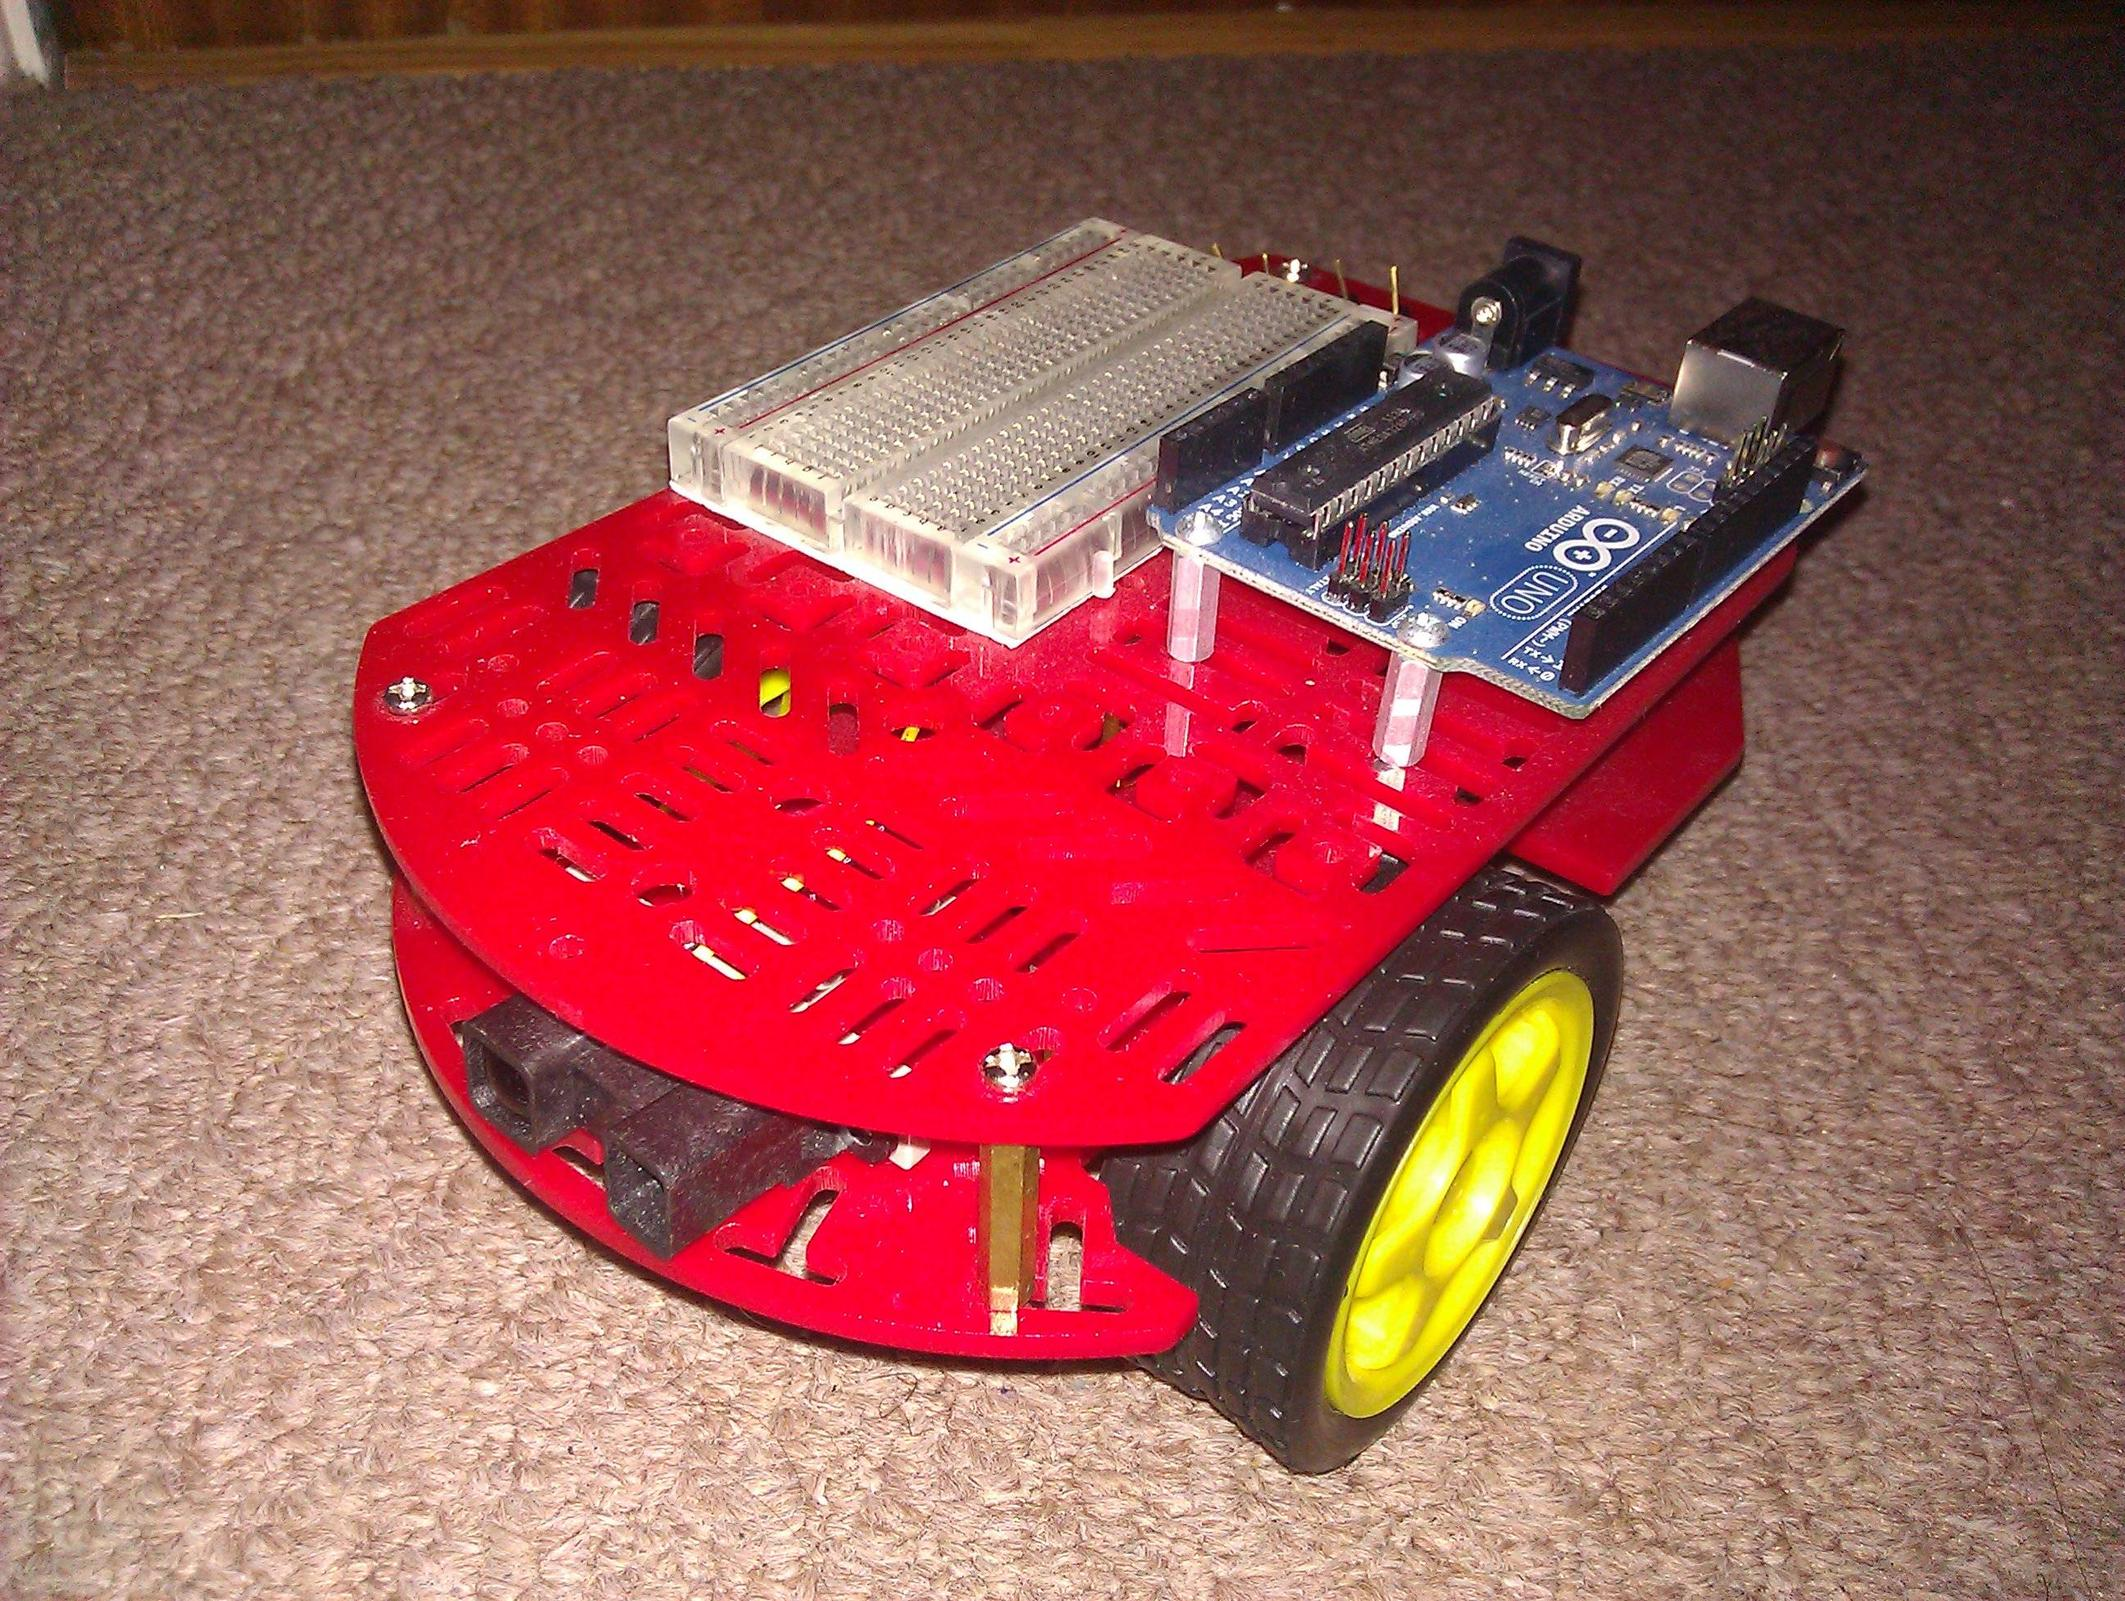
\includegraphics[width=3.0in] {Images/tria-mkI.jpg}
        \caption{Prototype mkI}
        \label{Prototype mkI}
\end{figure}

\begin{lstlisting}[language=c++]
if(sensor_range < value)
{
	motors.turn(random);
}else
{
	motors.forward(1);
}
\end{lstlisting}
